\section{Speed of Sound vs. the Speed of Baseballs}
%By Matt Trawick.

\makelabheader %(Space for student name, etc., defined in master.tex)

\bigskip

\textbf{Objective:}

In this lab, you'll explore how the speed of a wave (like sound) is different from the speed of a particle (like a baseball).

\bigskip

\textbf{Activity 1: A Ride in a Limo}

Imagine you are sitting in the back of a very long stretch limousine parked in front of a theater, and you yell to your driver ``Okay, let's go, please!''  The sound travels from the back of the limousine to the front at the speed of sound, 343~m/s.

\begin{enumerate}[labparts]
\item Is there anything you could do to make the sound travel to the driver faster than the speed of sound?
\begin{itemize}
\item Could you yell louder?
\bigskip
\item Could you use a higher or lower voice?
\bigskip
\item Could you thrust your face forward quickly as you say each word?
\bigskip
\item If the limousine is long enough, could you run from the back towards the front as you yelled?
\bigskip
\end{itemize}
%\answerspace{0.8in}

Once the sound waves leave your mouth, what happens to the sound waves only depends on the air itself.  The speed of sound could vary with the pressure or the temperature of the air, but nothing you do with your mouth can change how fast the sound travels through the air.  In this scenario, you are the ``source'' of the waves, and the air is the ``medium'' which carries the waves.  The speed of sound waves is not affected by the speed of the source.

\medskip
\item The limousine drives forward at 10~m/s, and you sit back to enjoy the ride.  But the windows are closed, and it's getting hot inside.  You ask the driver, ``Can you please turn on the air conditioning?''
In the reference frame of the limousine, what is the speed of the sound inside the cabin?  \textit{(Hint: Remember the principle of Galilean relativity, that the laws of mechanics are the same in all reference frames!)}
\answerspace{0.8in}

\item As you continue down the street at 10~m/s, you approach two police officers directing traffic.   If you speak to your driver again, how fast would the sound waves inside the limousine travel in the reference frame of the police officers?  (That is, if the officers could \textit{see} the sound waves, how fast would they see the sound waves coming towards them?)
\answerspace{0.8in}
\end{enumerate}

\pagebreak[3]
\textbf{Activity 2: Taking Away the Walls}

So far, we've imagined sound traveling within the closed cabin of a limousine.  But does the closed cabin of the limousine really change anything?  Do the air molecules carrying the sound know about the walls of the limousine?  Let's take another example.
\begin{enumerate}[labparts]

\item You and your friend are skateboarding down the street at 10~m/s, with your friend ahead of you.  But the wind is blowing at 10~m/s in the same direction as you are going, so you feel no wind in your face.  If you yell to your friend ahead of you, how fast does the sound travel in your reference frame? \textit{(Hint: think back to the limo!)}
%\answerspace{0.4in}

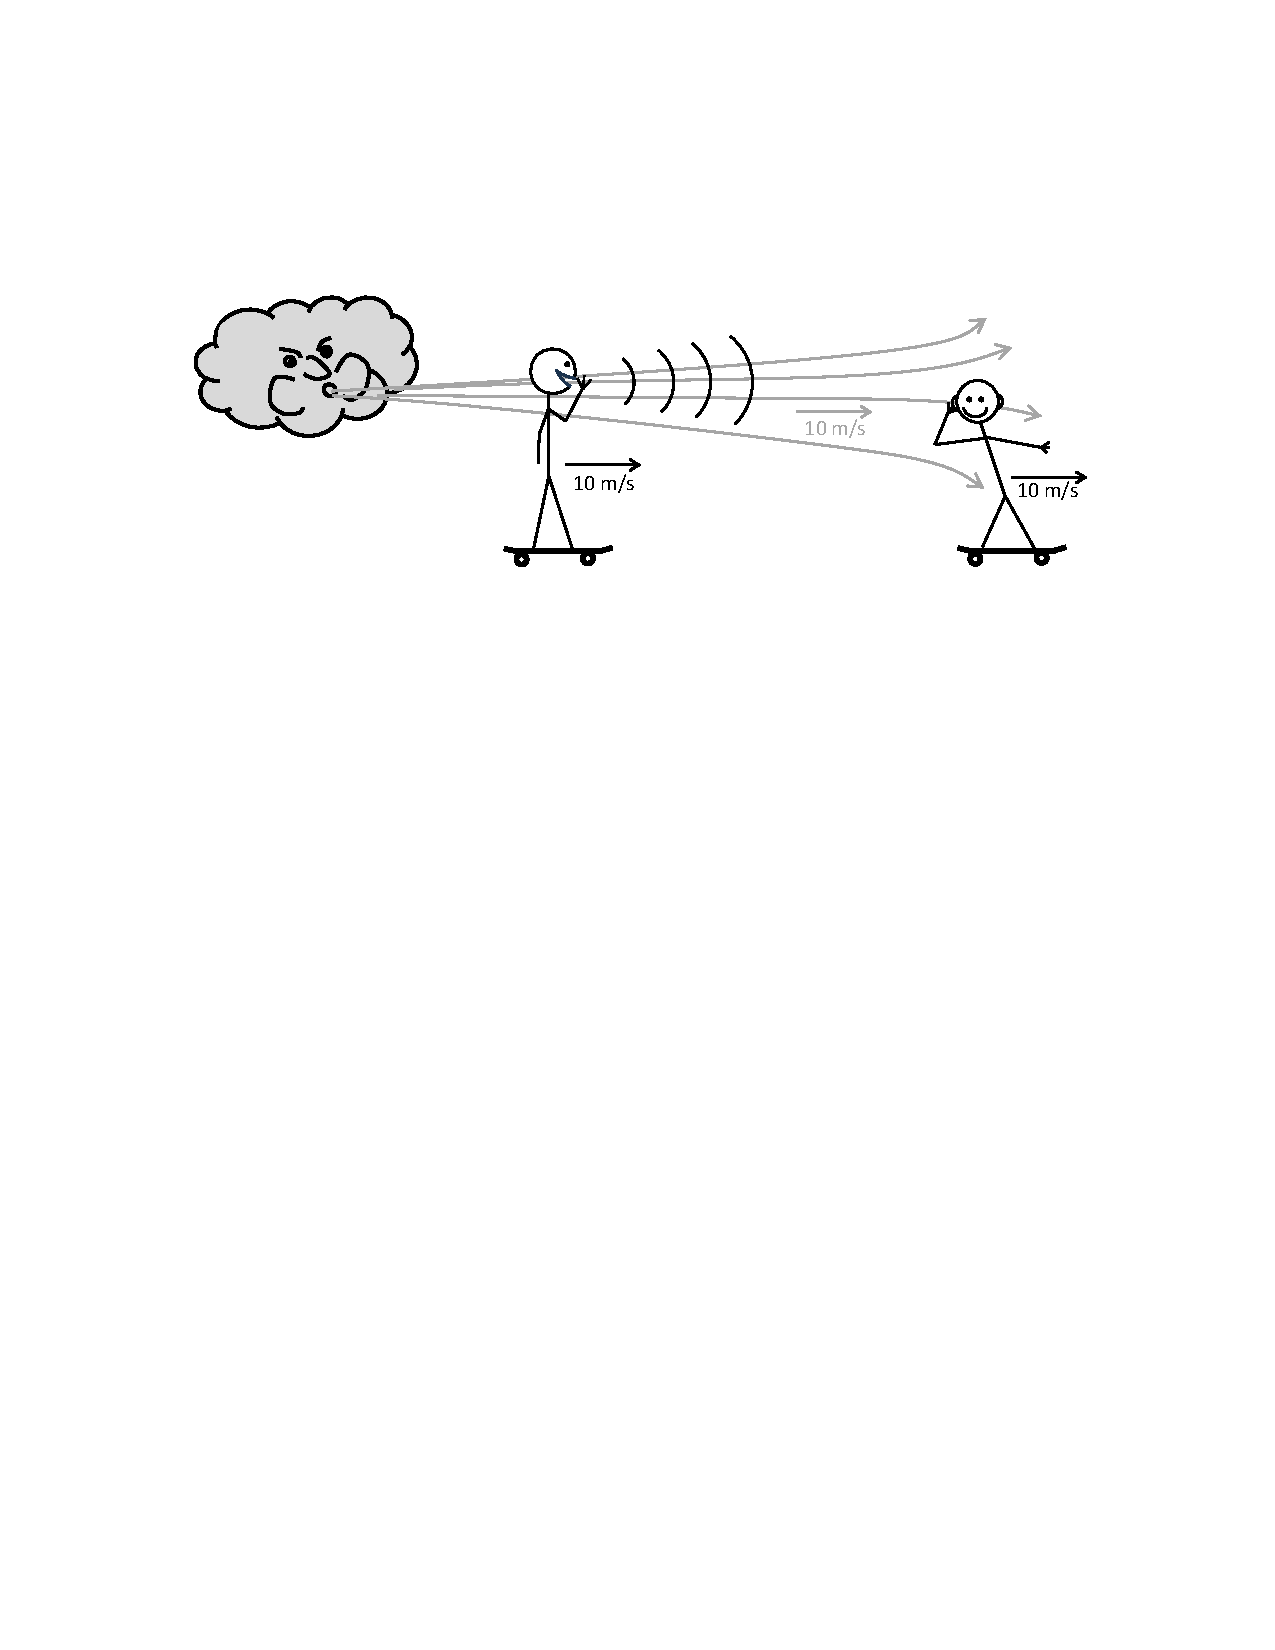
\includegraphics[scale=0.6]{sound_vs_baseballs/skateboarders1.pdf}

\item If you approach the same pair of police officers as before, how fast is the sound traveling towards them in the police officers' reference frame? \textit{(Hint: again, think back to the limo!)}
%\answerspace{0.4in}

\hspace{\fill}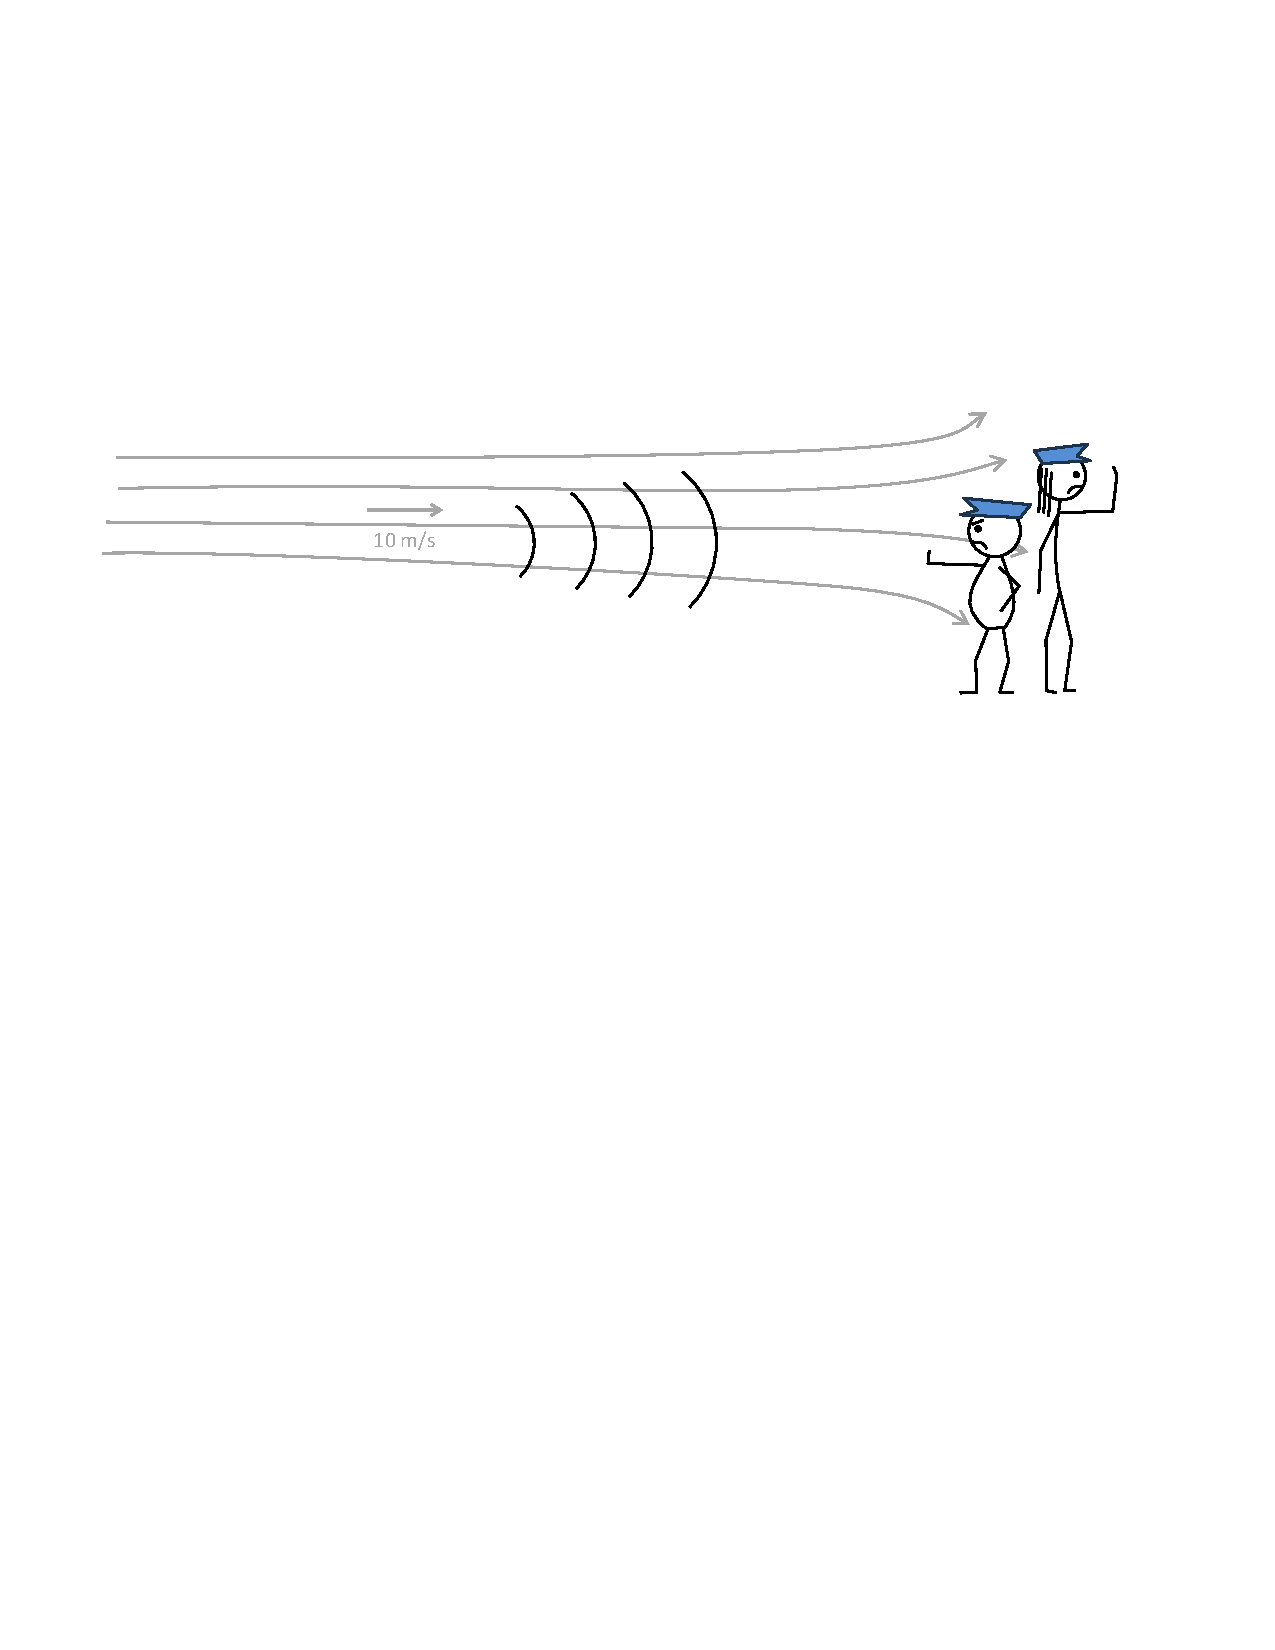
\includegraphics[scale=0.6]{sound_vs_baseballs/skateboarders2.pdf}
\index{color page}

\item Now you and your friend stop, and you yell to your friend again.  But the wind is still blowing at 10~m/s towards the police officers.  Now how fast does the sound travel towards the police in the reference frame of the police officers?
\answerspace{0.3in}

\hspace{\fill}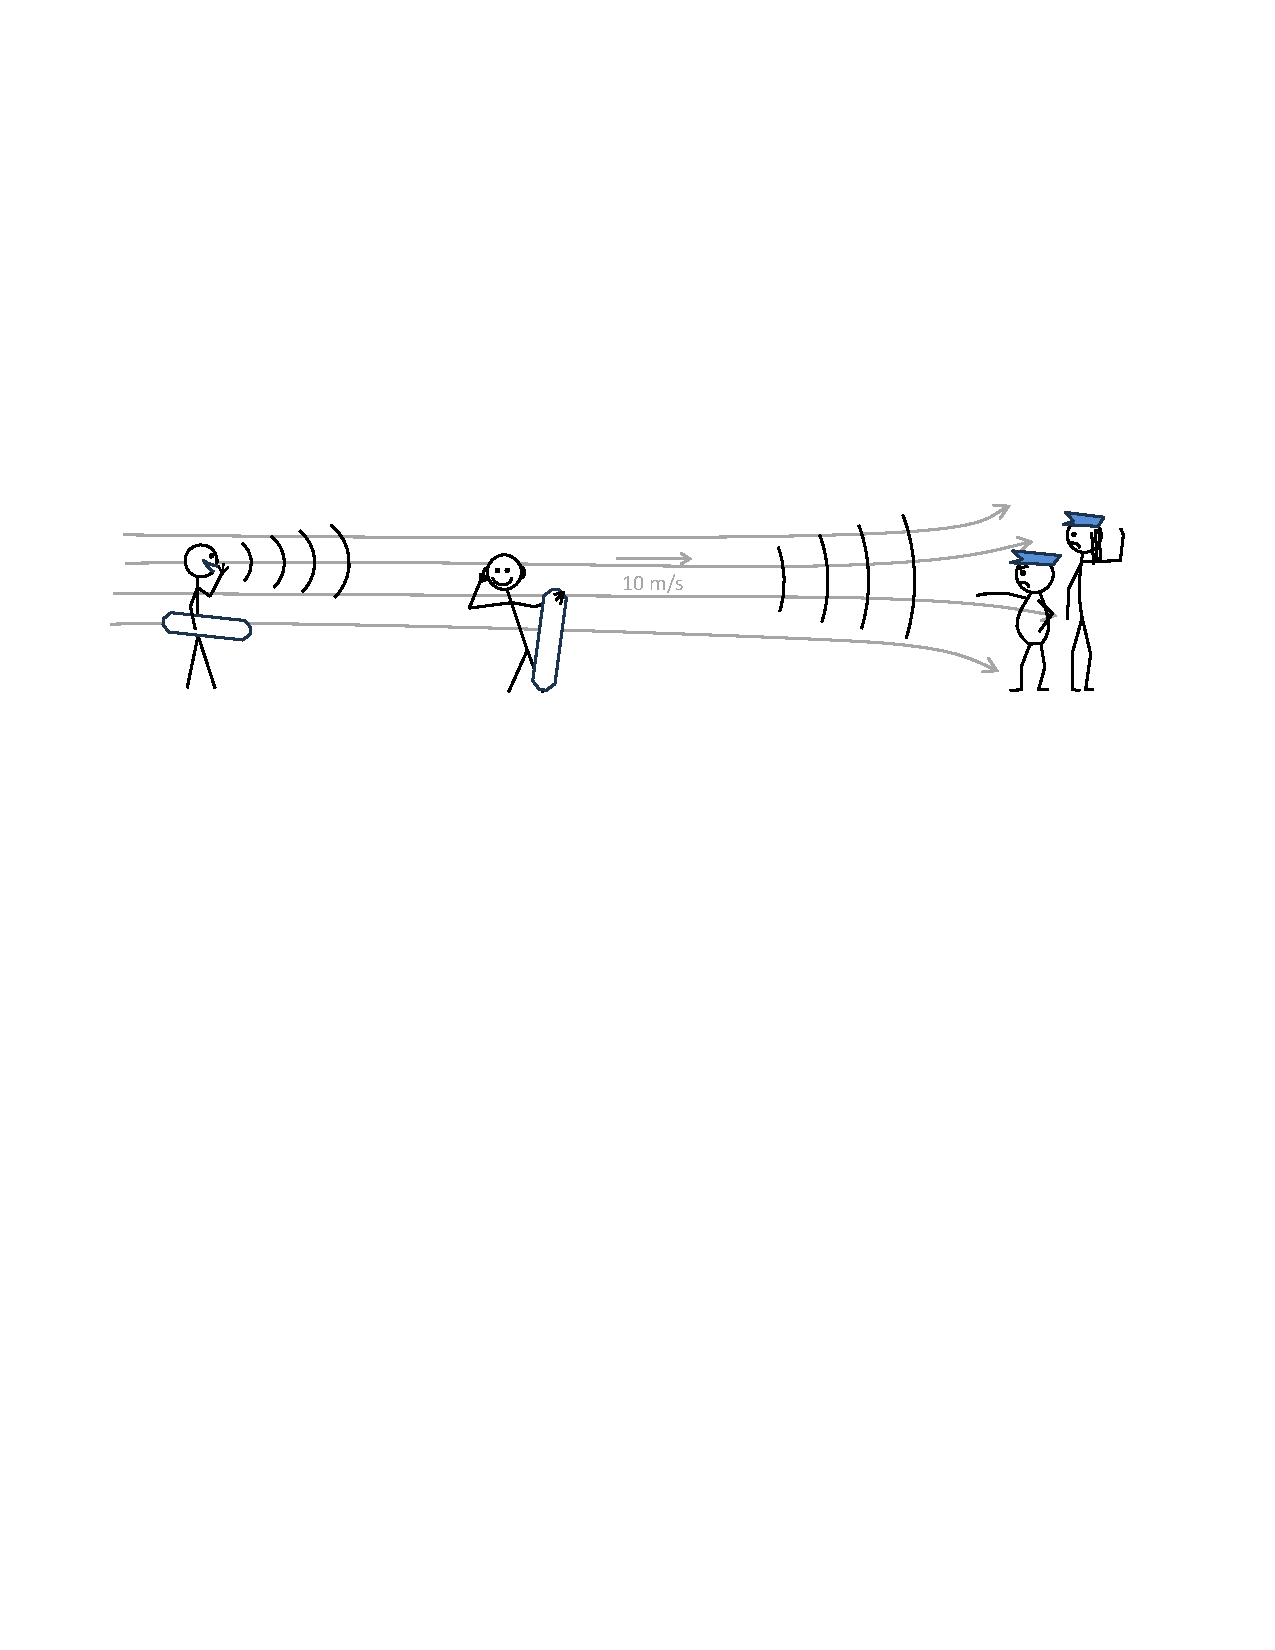
\includegraphics[scale=0.8]{sound_vs_baseballs/skateboarders3.pdf}
\index{color page}

\item If you are still stopped and the wind still blows at 10~m/s, but the police officers run towards you at 5~m/s, now how fast is the sound in the reference frame of the officers?
\answerspace{0.1in}

\begin{center}
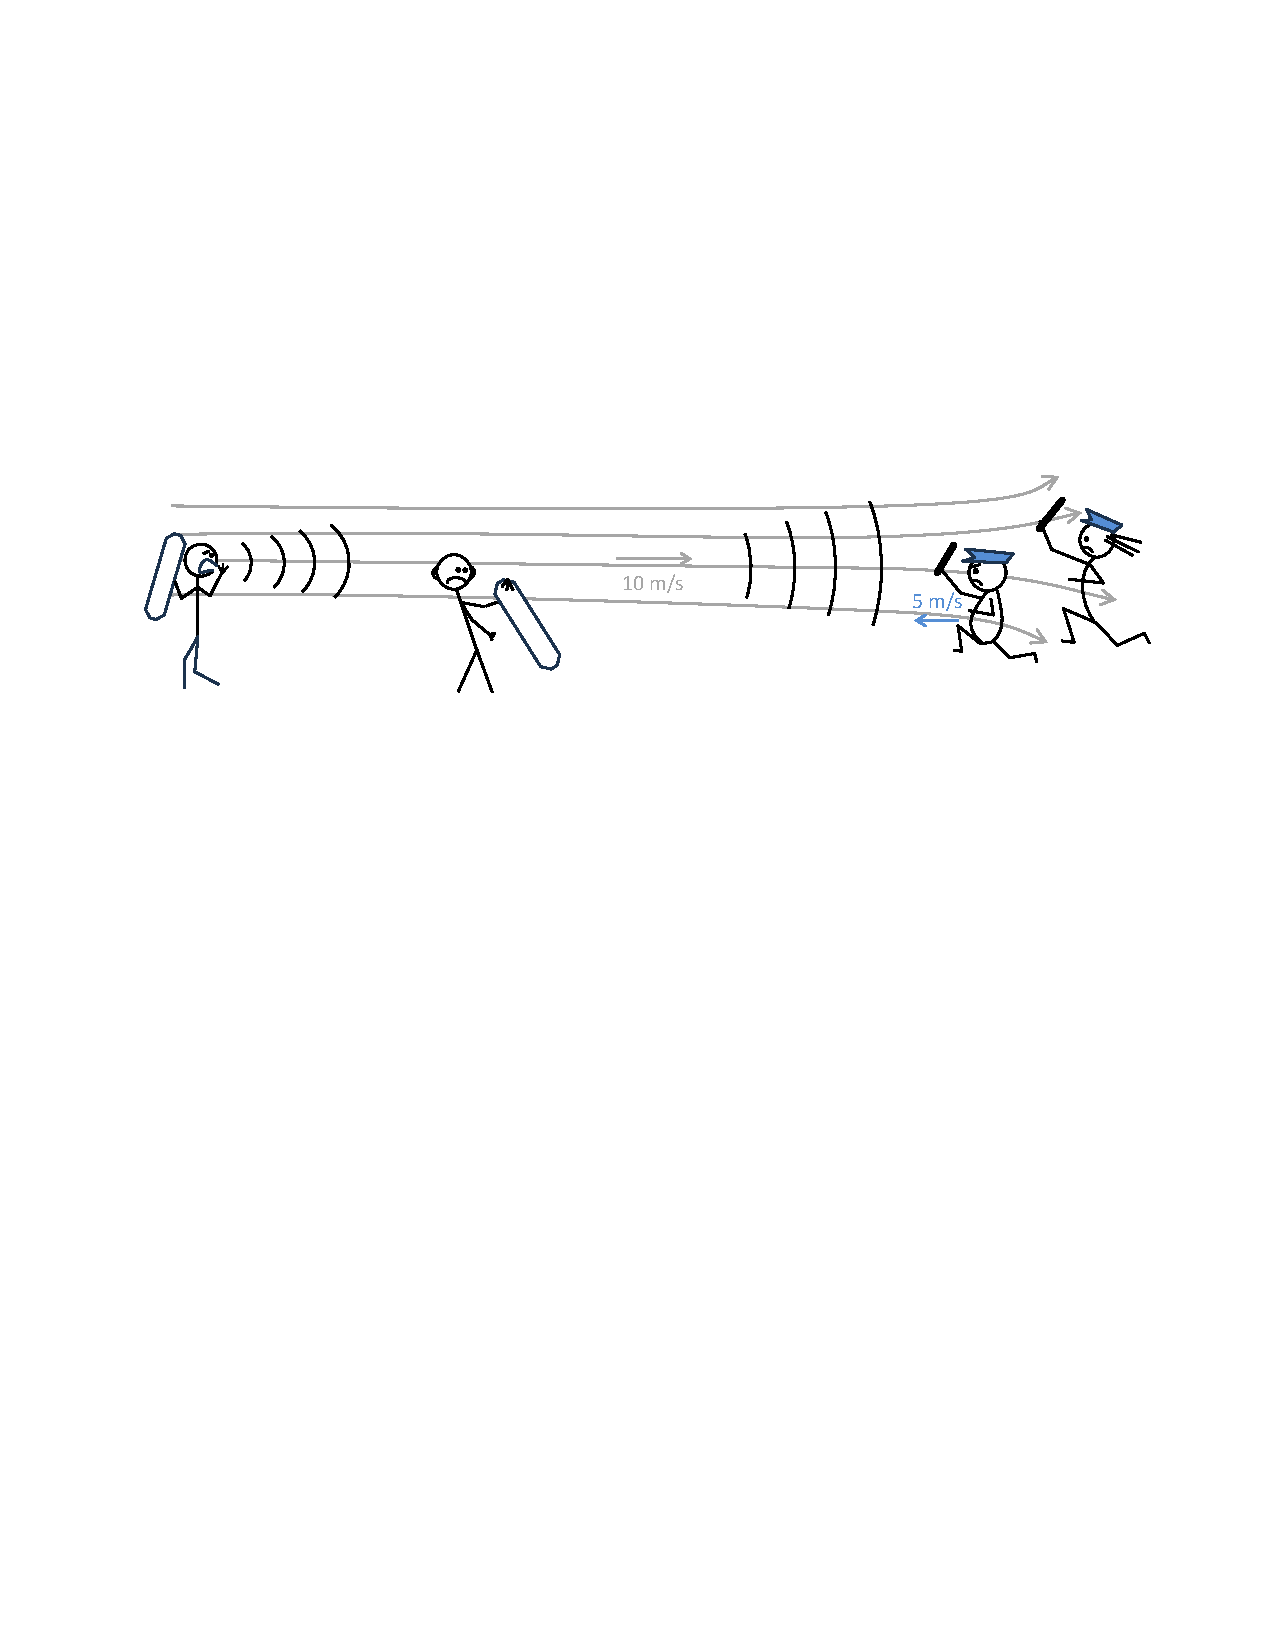
\includegraphics[scale=0.8]{sound_vs_baseballs/skateboarders4.pdf}
\index{color page}
\end{center}

\textit{This last question is important. It's not just just the speed of the wind (relative to the Earth, say) that matters.  
What matters is the speed of the wind \underline{relative to the police officers.}}
\medskip

\item Remember, the source of the sound is you yelling, and the medium for the sound waves is the air.  The ``receiver'' of the sound is the limo driver, your friend, or (in this case) the police officers.  Let's summarize what determines the speed of the sound waves in the police officers' reference frame:
\begin{itemize}
\item Does the speed of sound waves depend on the speed of the \textit{medium}, relative to the receiver?
\answerspace{0.5in}
\item Does the speed of sound waves depend on the speed of the \textit{source}, relative to the receiver?
\answerspace{0.5in}
\end{itemize}
\end{enumerate}

\pagebreak[3]
\textbf{Activity 3: Particles}

A baseball is not a wave, of course; it's a solid object, or a ``particle.''  
Where the speed of sound waves in air is constant (always 343~m/s relative to the air), the speed of a baseball in air can vary, because it depends on how fast you throw the baseball.  Put another way, the speed of a baseball doesn't depend on the speed of the medium.\footnote{It's a little tricky, because air drag \textit{does} slow a baseball down a little bit, but it's very different from sound waves.  We saw that a 10~m/s wind can automatically make sound travel at 353~m/s.  But a 10~mph wind doesn't automatically turn a 90~mph fastball into a 100~mph fastball.}  
In fact, baseballs don't even need a medium; you could throw a baseball just fine in outer space.

\begin{enumerate}[labparts]
\item Suppose you are throwing a baseball to your friend, as hard as you can, at 50~mph in your reference frame.  What is the speed of the baseball in your friend's reference frame\ldots
\begin{itemize}
\item {\ldots}if your friend is traveling towards you on a train car at 10 mph?
\answerspace{0.2in}

\item {\ldots}if your friend is standing still on the tracks, but you are traveling towards your friend on a train car at 10 mph?
\answerspace{0.2in}

\item {\ldots}if you and your friend are both on train cars, with a relative speed towards each other of 20 mph?
\answerspace{0.2in}
\end{itemize}

\item Here, the ``source'' of the particle is you, and the receiver is your friend.  Summarize what determines the speed of a particle in the your friend's reference frame:
\begin{itemize}
\item Does the speed of a particle depend on the speed of any \textit{medium}, relative to the receiver (bearing in mind that the correct answer is ``no'')?
\answerspace{0.5in}
\item Does the speed of a particle depend on the speed of the \textit{source}, relative to the receiver?
\answerspace{0.5in}
\end{itemize}

\end{enumerate}

\pagebreak[3]
\textbf{Activity 4: What About Light?}

We've said previously that light behaves like both a particle and a wave. 
\begin{enumerate}[labparts]
\item Do you think the speed of light depends on the speed of the source, relative to the receiver?  Explain.
\answerspace{0.8in}

\item How could you test it experimentally?
\answerspace{0.8in}

\item Do you think the speed of light depends on the speed of the medium, relative to the receiver?  Explain.
\answerspace{0.8in}

\item How could you test it experimentally?
\answerspace{0.8in}

\end{enumerate}


